\chapter{Casi d'uso}\label{casiDuso}
In questo capitolo vengono elencati i casi d'uso individuati per il progetto GDP in accordo con il proponente. Ogni caso d'uso indica un'interazione tra uno o più attori e il sistema. Questa interazione genera uno scenario che è l'insieme delle azioni che hanno in comune uno scopo finale per un utente.

\section{Casi d'uso tra un utente ed il front end}
%spiegazione della sezione
\subsection{Attori dei casi d'uso}
\begin{center}
	\begin{figure}[H]
		
\includegraphics{../immagini/attori_casi/utente_generico.png}
		\caption{Attore: utente generico}
	\end{figure}
\end{center}
\subsubsection{Attori Primari}\label{UFattoriPrimari}
\begin{itemize}
	\item \textbf{Utente generico:} definisce l'utente generico che utilizza l'applicazione web;
\end{itemize}

\subsection{Elenco casi d'uso}\label{UFelencoCasiDuso}

\subsubsection{UC1 - Visualizzazione informazioni sulla mappa} \label{visualizzazioneInfoMappa} %parzialmente corretto
\begin{center}
	\begin{figure}[H]
		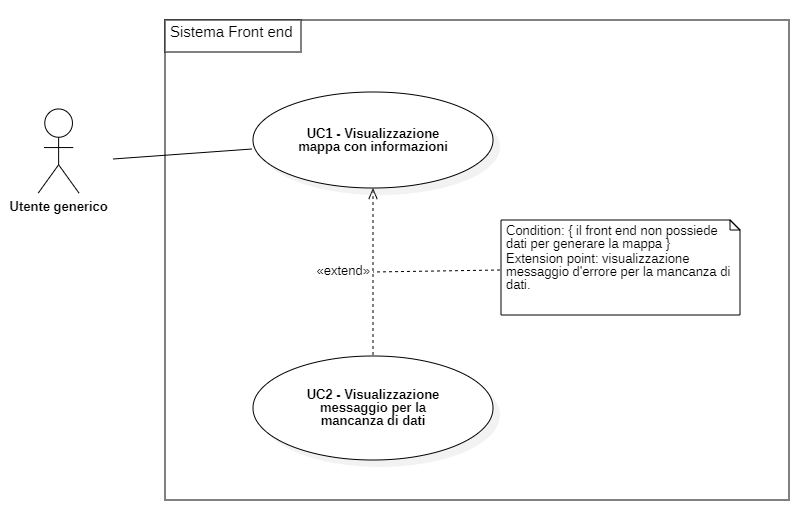
\includegraphics[scale=0.8]{../immagini/attori_casi/uc1_uc2.png}
		\caption{UC1 - Visualizzazione informazioni sulla mappa}
	\end{figure}
\end{center}
\begin{itemize}
	\item \textbf{Attori primari}: utente generico;
	\item \textbf{Descrizione}: l’utente accede all’applicazione web e visualizza la heat map$_{\scaleto{G}{3pt}}$. La mappa mostra la città impostata di default o quella selezionata tra quelle a disposizione, come definito nell’UC3(). Le informazioni vengono ricavate dall’orario e la data impostate dall’utente come indicato nel UC4.1() e UC4.2() o si utilizzano i dati in tempo reale quindi usando l’orario attuale;
	\item \textbf{Scenario principale}: L’utente accede all’applicazione web e visualizza la heat map$_{\scaleto{G}{3pt}}$ della città;
	\item \textbf{Precondizione}: il front end può generare la mappa, la città, la data, l’ora sono state indicate dall’utente o vengono utilizzate quelle di default, quindi data e ora sono quelle odierne di sistema per dati in tempo reale;
	\item \textbf{Postcondizione}: l’utente visualizza la heat map$_{\scaleto{G}{3pt}}$ con i dati ricavati nell’istante di tempo selezionato, come definito nell’UC4 (\S~\ref{impostazioneIstanteTempo}), e alla città scelta fra quelle disponibili come descritto nella definizione dell’UC3 (\S~\ref{selezioneCitta}), oppure visualizza quella riguardante la città impostata di default;
	\item \textbf{Estensioni}: l’utente accede all’applicazione web, il front end rilevando la richiesta di generazione della mappa individua una mancanza di dati per la sua costruzione e di conseguenza viene visualizzato un messaggio relativo all’errore riscontrato (UC2 \S~\ref{visualizzazioneMessaggioMancanzaDati});
\end{itemize}

\subsubsection{UC2 - Visualizzazione messaggio per la mancanza di dati }\label{visualizzazioneMessaggioMancanzaDati} %parzialmente corretto
\begin{itemize}
	\item \textbf{Attori primari}: utente generico;
	\item \textbf{Descrizione}: l’utente visualizza un messaggio d’errore per la mancanza di dati necessari alla generazione della mappa. Questo accade quando il front end non ha a disposizione tutti i dati;
	\item \textbf{Scenario principale}: 
	\begin{itemize}
		\item L’operazione di generazione mappa fallisce;
		\item L’utente visualizza un messaggio di errore per la mancanza dei dati;
		\item L’utente clicca il pulsante “ok” per chiudere il messaggio.
	\end{itemize}
	\item \textbf{Precondizione}: il front end effettua un controllo sui dati, non sono presenti tutti i dati;
	\item \textbf{Postcondizione}: viene visualizzato un messaggio all’utente per informarlo sul problema riscontrato e l’operazione fallisce.
\end{itemize}

\subsubsection{UC3 - Selezione città da visualizzare nella mappa}\label{selezioneCitta} 
\begin{center}
	\begin{figure}[H]
		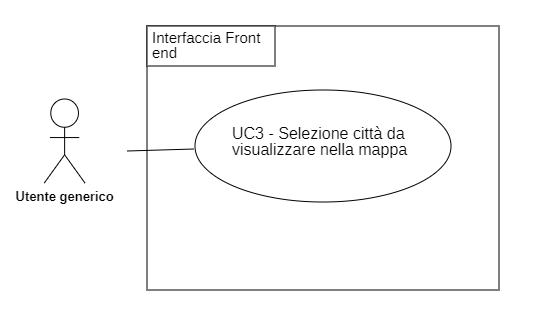
\includegraphics{../immagini/attori_casi/uc3.png}
		\caption{UC3 - Selezione città da visualizzare nella mappa}
	\end{figure}
\end{center}
\begin{itemize}
	\item \textbf{Attori primari}: utente generico;
	\item \textbf{Descrizione}:  l’utente può selezionare la città di cui vuole visualizzare la heat map$_{\scaleto{G}{3pt}}$;
	\item \textbf{Scenario principale}:l’utente seleziona una città tra quelle messe a disposizione;
	\item \textbf{Precondizione}: il sistema dispone di informazioni relative a diverse città;
	\item \textbf{Postcondizione}:   l’utente ha selezionato la città che vuole visualizzare, la heat-map$_{\scaleto{G}{3pt}}$ si aggiorna in base alla scelta fatta.
\end{itemize}

\subsubsection{UC4 - Impostazione dell’istante di cui visualizzare la heat map$_{\scaleto{G}{3pt}}$
} \label{impostazioneIstanteTempo}%parzialmente corretto
\begin{center}
	\begin{figure}[H]
		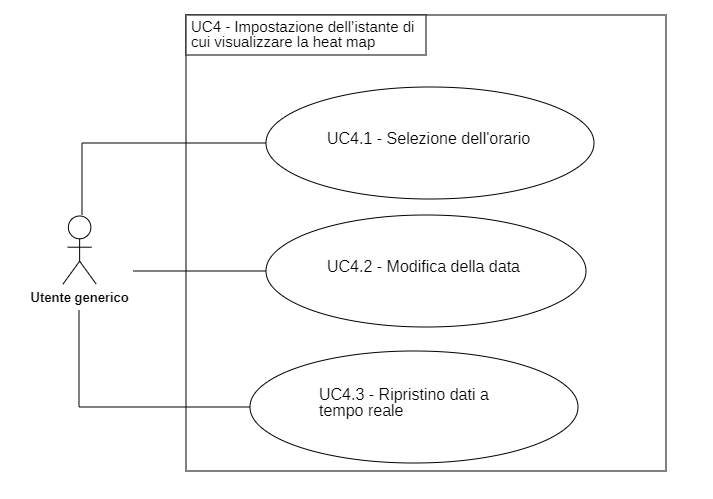
\includegraphics{../immagini/attori_casi/uc4.png}
		\caption{UC4 - Impostazione dell’istante di cui visualizzare la heat map}
	\end{figure}
\end{center}
\begin{itemize}
	\item \textbf{Attori primari}: utente generico;
	\item \textbf{Descrizione}: l’utente attraverso l’interfaccia del sistema, modifica l’istante di tempo di cui vuole visualizzare i dati;
	\item \textbf{Scenario principale}: attraverso l’interfaccia l’utente può decidere di:
		\begin{enumerate}
			\item Modificare l’orario dei dati da visualizzare (UC4.1 \S~\ref{selezioneOrario});
			\item Modificare il giorno tra quelli disponibili (UC4.2 \S~\ref{modificaData});
			\item Ritornare ai dati in tempo reale (UC4.3 \S~\ref{ripristinoTempoReale}).
		\end{enumerate}
	\item \textbf{Precondizione}: il sistema dispone di informazioni su diversi istanti di tempo;
	\item \textbf{Postcondizione}: l’utente ha selezionato un istante di tempo diverso da quello di default e visualizza i dati riguardanti ad esso.%insicuro
\end{itemize}

\subsubsection{UC4.1 - Selezione dell’orario}\label{selezioneOrario}
\begin{itemize}
	\item \textbf{Attori primari}: utente generico;
	\item \textbf{Descrizione}: l’utente seleziona un orario diverso da quello attuale per visualizzare i dati di quel momento;
	\item \textbf{Scenario principale}: l’utente imposta un orario utilizzando l’interfaccia dell’applicazione web;
	\item \textbf{Precondizione}: il sistema ha informazioni riguardanti tutti i diversi orari; %insicuro
	\item \textbf{Postcondizione}:  l’orario viene aggiornato e la mappa visualizza i dati della modifica fatta.
\end{itemize}

\subsubsection{UC4.2 - Modifica della data}\label{modificaData}
\begin{itemize}
	\item \textbf{Attori primari}: utente generico;
	\item \textbf{Descrizione}: l’utente seleziona una data diversa da quella odierna e tra quelle disponibili e visualizza la mappa della data scelta;
	\item \textbf{Scenario principale}: l’utente seleziona una data diversa da quella attuale;
	\item \textbf{Precondizione}: il sistema possiede informazioni su tutte le date fino a quella odierna;
	\item \textbf{Postcondizione}: l’utente visualizza l’heat map$_{\scaleto{G}{3pt}}$ aggiornata con i dati del giorno selezionato all’orario attuale o all’orario scelto dall’utente stesso secondo quanto definito nella descrizione dell’UC4.1 (\S~\ref{selezioneOrario}).
\end{itemize}

\subsubsection{UC4.3 - Ripristino dati a tempo reale}\label{ripristinoTempoReale}
\begin{itemize}
	\item \textbf{Attori primari}: utente generico;
	\item \textbf{Descrizione}:  l’utente sceglie di osservare i dati in tempo reale;
	\item \textbf{Scenario principale}: l’utente preme sul pulsante per il ripristino dei valori attuali di data e ora;
	\item \textbf{Precondizione}: l’utente ha impostato una data e/o un’ora diversa dal valore di quella attuale (UC4.1 \S~\ref{selezioneOrario} e UC4.2 \S~\ref{modificaData});
	\item \textbf{Postcondizione}: l’utente visualizza la mappa con i dati in tempo reale.
\end{itemize}

\section{Casi d'uso tra il front end ed il back end}\label{ucFrontEndBackEnd}
%spiegazione sezione

\subsection{Attori dei casi d'uso} %immagine errata
\begin{center}
	\begin{figure}[H]
		
\includegraphics{../immagini/attori_casi/sistema_front_end.png}
		\caption{Attore: Sistema front end}
	\end{figure}
\end{center}
\subsubsection{Attori Primari}\label{FBattoriPrimari}
\begin{itemize}
	\item \textbf{Sistema front end:} Definisce una parte del sistema sviluppato che interagisce con il sistema back end;
\end{itemize}

\subsection{Elenco casi d'uso}\label{FBelencoCasiDuso}


\subsubsection{UC5 - Richiesta dati al back end}\label{richiestaDati}
\begin{center}
	\begin{figure}[H]
		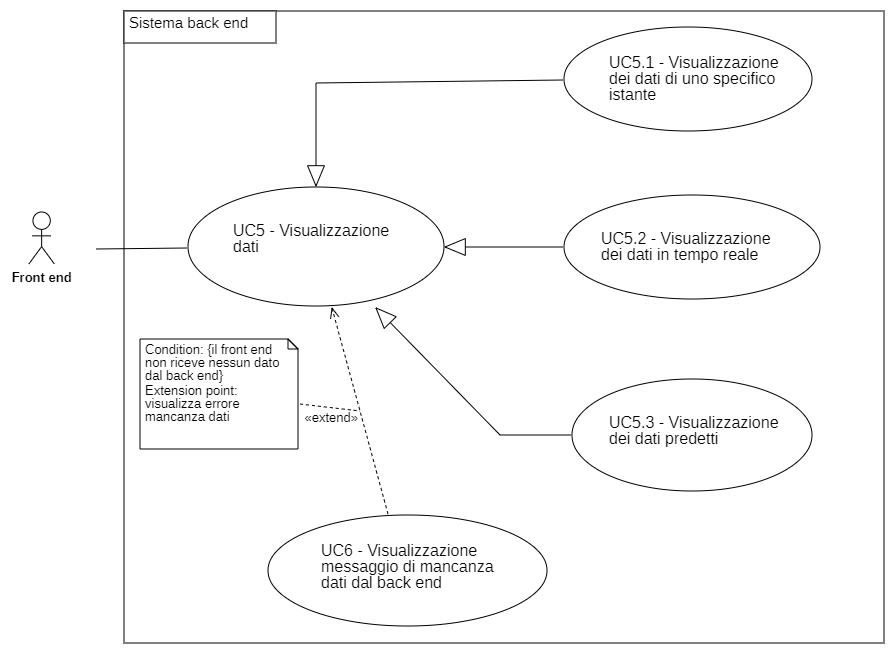
\includegraphics[scale=0.7]{../immagini/attori_casi/uc5_uc51_uc52_uc53.png}
		\caption{UC5 - Richiesta dati al back end}
	\end{figure}
\end{center}
\begin{itemize}
	\item \textbf{Attori primari}: sistema front end;
	\item \textbf{Descrizione}: il front end richiede dati al backend per generare la heat-map$_{\scaleto{G}{3pt}}$;
	\item \textbf{Scenario principale}: il front end richiede al back end le informazioni necessarie alla generazione della heat map$_{\scaleto{G}{3pt}}$;
	\item \textbf{Precondizione}: il front end non ha le informazioni per poter generare la mappa;
	\item \textbf{Postcondizione}: Il front visualizza e riceve le nuove informazioni. 
	\item \textbf{Generalizzazioni}: il front end può fare una delle seguenti richieste:
	\begin{itemize}
		\item Richiede i dati di uno specifico istante (UC5.1\S~\ref{richiestaDatiGiorno});
		\item Richiede i dati in tempo reale (UC5.2 \S~\ref{richiestaDatiTempoReale});
		\item Richiede i dati predetti (UC5.1 \S~\ref{richiestaDatiPredetti}).
	\end{itemize}
	\item \textbf{Estensione}: il front end effettua la richiesta al back end, il back end non invia nessun dato nella risposta (UC6 \S~\ref{VisualizzazioneMancanzaBackEnd} )
\end{itemize}

\subsubsection{UC5.1 - Richiesta dati di uno specifico istante}\label{richiestaDatiGiorno}
\begin{itemize}
	\item \textbf{Attori primari}: sistema front end;
	\item \textbf{Descrizione}: Il front end richiede le informazioni relative ad uno specifico istante di tempo;
	\item \textbf{Scenario principale}:  il front end richiede al back end le informazioni relative all'istante di tempo specificato;
	\item \textbf{Precondizione}: L’utente esegue la modifica della data o dell’orario come definito rispettivamente nella descrizione di UC4.2 (\S~\ref{modificaData}) e UC4.1 (\S~\ref{selezioneOrario}) ponendo un orario precedente a quello odierno;
	\item \textbf{Postcondizione}: Il front end visualizza e riceve le informazioni relative all'istante di tempo impostato. 
\end{itemize}

\subsubsection{UC5.2 - Richiesta dei dati in tempo reale}\label{richiestaDatiTempoReale}
\begin{itemize}
	\item \textbf{Attori primari}: sistema front end;
	\item \textbf{Descrizione}: il front end richiede i dati reali più recentemente aggiunti;
	\item \textbf{Scenario principale}: il front end richiede al back end le informazioni più recentemente aggiunte;
	\item \textbf{Precondizione}: Viene eseguita la visualizzazione della mappa come definito nell’UC1 (\S~\ref{visualizzazioneInfoMappa}) o avviene il ripristino dei dati in tempo reale come definito in UC4.3 (\S~\ref{ripristinoTempoReale});
	\item \textbf{Postcondizione}: Il front end ha ricevuto i dati ed è pronto alla generazione della heat map$_{\scaleto{G}{3pt}}$. 
\end{itemize}

\subsubsection{UC5.3 - Richiesta dati predetti}\label{richiestaDatiPredetti}
\begin{itemize}
	\item \textbf{Attori primari}: sistema front end;
	\item \textbf{Descrizione}: il front end richiede i dati riferiti allo stesso giorno ma ad un orario avanzato rispetto a quello attuale.
	I dati sono ricavati dall’elaborazione, attraverso un modello di machine learning$_{\scaleto{G}{3pt}}$, dei dati reali acquisti;
	\item \textbf{Scenario principale}: il front end richiede al back end i dati elaborati dal modello machine learning$_{\scaleto{G}{3pt}}$;
	\item \textbf{Precondizione}: le informazioni vengono visualizzate sulla mappa come definito nell’UC1 (\S~\ref{visualizzazioneInfoMappa}), impostando un orario successivo a quello attuale come descritto nell’UC4.1 (\S~\ref{selezioneOrario});
	\item \textbf{Postcondizione}: il front end ha ricevuto i dati ed è pronto alla generazione della heat map$_{\scaleto{G}{3pt}}$. 
\end{itemize}

\subsubsection{UC6 - Visualizzazione messaggio di mancanza dati dal back end}\label{VisualizzazioneMancanzaBackEnd}
\begin{itemize}
	\item \textbf{Attori primari}: sistema front end;
	\item \textbf{Descrizione}: il front end riceve un messaggio di mancanza dati rispetto alla richiesta data;
	\item \textbf{Scenario principale}: 
	\begin{enumerate}
		\item il front end richiede dei dati specifici al back end;
		\item la risposta ricevuta è un messaggio di errore;
		\item il front end ritenta la richiesta di informazioni. 
	\end{enumerate}
	\item \textbf{Precondizione}: il front end effettua una richiesta di dati, il back end non ha a disposizione i dati richiesti;
	\item \textbf{Postcondizione}: il front end riceve un messaggio di errore per la mancanza dei dati richiesti. 
\end{itemize}

